\documentclass[12pt, letterpaper]{article}

\usepackage{times} % for Times font

%\usepackage{forest} % for linguistic trees
%\usepackage{elocalloc} % -> Require package elocalloc for local boxes for the forest package
\usepackage{tikz} % for linguistic trees
\usepackage{tikz-qtree, ,tikz-qtree-compat} % for linguistic trees
\tikzset{every tree node/.style={align=center, anchor=north}}% set up the arrows 
\usepackage{tipa} % package for ipa
\usepackage{phonrule} % package for phonology rule 


\usepackage{amsmath}	% for semantic representation
\usepackage{stmaryrd}	% for semantic representation [[ ]]
\newcommand{\evaluation}[2][]{\ensuremath{\llbracket #2\rrbracket^{#1}}}	% semantic representation [[ ]]

\usepackage{gb4e} % for linguistic examples
\let\eachwordone=\it % first gloss line in italics in gb4e

\begin{document}

\title{LIN 300  \LaTeX~ tutorial}
\author{Hongchen Wu (Put your name instead)}
% If you omit \date{}, it will show today's date.
\maketitle

\begin{enumerate}
	\item This is a \LaTeX~template for linguistic writing in general.

	\item The advantages of \LaTeX~(in comparison with MS Word):
		\begin{enumerate}
			\item It is free.

			\item The output looks beautiful.
			
			\item It automatically numbers examples and aligns glosses.
			
				\begin{exe}
				\ex\label{example} This is an example.
				\ex\label{english example} \begin{xlist}
				        \ex\label{ex a} This is an English example.
				        \ex\label{ex b} This is a longer English example.
				    \end{xlist}
				
				\ex\label{korean example} This is a Korean example. \gll 
					Nwukwu-na ku mwuncey-lul phwu-ess-ta.\\
					who-\textsc{na} that problem-\textsc{acc} solve-\textsc{past}-\textsc{decl}\\
					\glt `Everyone solved that problem.'
				\end{exe}
						
			\item Cross-referencing examples is easier. \\

				As shown in the example (\ref{ex b}), ...\\

			\item \LaTeX files are plain text files so they are smaller in size.
			
			\item You can write semantic equations more easily.\\
%% for math symbolrs you can check this refernece.  Google "latex math symbols"
%http://web.ift.uib.no/Teori/KURS/WRK/TeX/symALL.html

				\evaluation{X\mbox{-}na \ Q} = $ \forall x_i [(x_i \in X) \supset Q(x_i)] $ \\
																			where X = $ \{x_1, x_2, \cdots x_n\} $\\

                                 %predicate logic. 
                                $\exists x [white(x) \& dog(x)]$ \\
                               $\forall x [linguist(x) \rightarrow know(x, $\LaTeX$)]$

			\item You can draw syntactic trees without worrying about how/where to draw the lines.\\

				\Tree	[.S
							[.NP 
								[.N John ] 
							]
							[.VP 
								[.V loves ]
								[.NP 
									[.N Mary ] 
								]
							]
						]\\

                       
                         \item You center a tree by using ``center'' command.
                            \begin{center}
                                  \Tree [.S [.NP LaTeX ] [.VP [.V is ] [.NP fun ] ] ]
                            \end{center}
                            


                          \item You can draw tree with movement\\
%% add tree-packages 
%\usepackage{tikz-qtree, ,tikz-qtree-compat} % for linguistic trees
%\tikzset{every tree node/.style={align=center, anchor=north}}% set up the arrows 
                         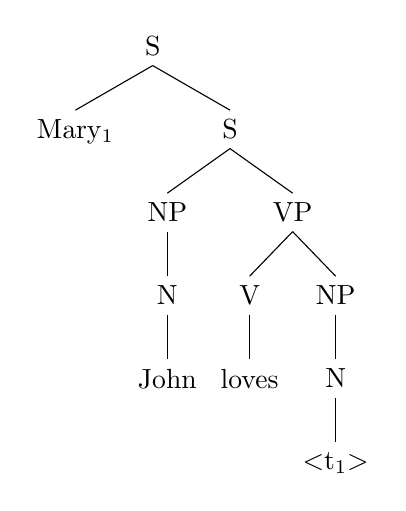
\begin{tikzpicture} % this means that you can call command for drawing curves
                             \Tree	[.S
                                             [.\node(M){Mary_1}; ]
                                             [.S
							[.NP 
								[.N John ] 
							]
							[.VP 
								[.V loves ]
								[.NP 
									[.N \node(Mtrace){$<$t_1$>$}; ] 
								]
							]
						]
                                        ]\\
                            % \draw[->] (Mtrace) [in=-90,out=-90,looseness=1.5]  to (M); %you also can assgin looseness=1.0 or 0.5. It depends on you.
                             %\draw[->] (Mtrace) [in=-120,out=-100,looseness=1, red]  to (M); % you also can change the color of the row
                              %\draw[->] (Mtrace) [in=-120,out=-100,looseness=1, dashed,red]  to (M); you also can change the shape of the row
                         \end{tikzpicture}

 
                      \item You can make cool IPA fonts in \LaTeX{} with the \textit{tipa} package.\\
 % add packages for ipa
% \usepackage{tipa}
                             \begin{center}
                                  \textipa{abcdefghijklmnopqrstuvwxyz}          \\
                                       \textipa{ABCDEFGHIJKLMNOPQRSTUVWXYZ}\\    

                                      \textipa{! * + = ? . , / [ ] ( ) ` ' | ||}    \\   %% symbols
                                      \textipa{1234567890 @}                       \\  %% vowels
                                    \textipa{\;A \;B \;E \;G \;H \;I \;L \;R \;Y} \\  
                                    \textipa{\:d \:l \:n \:r \:s \:t \:z}         \\
                                     \textipa{\!b \!d \!g \!j \!G \!o} \\
                             \end{center} 

                          
                       \item You can make really pretty phonological rules too!\\
                            \begin{center}
%add package for phonology rule
% \usepackage{phonrule}
                               \phonb{\phonfeat{+stop \\ +consonant \\ +alveolar} }{\textipa{R}}{\phonfeat{+vowel \\ +stressed} }{\phonfeat{+vowel \\ +stressed} }\\
                                        \end{center}
                                 


                        \item You can draw a nice tabular with latex.\\
% create 5 rows with P ∧ R at the top separated by a
% horizontal line: hline
%let's creat a truth-table
                           \begin{tabular}{cc|ccc}
                                   p & q & p & $\wedge $ & q \\
                                   \hline
                                    T & T & T & T & T \\
                                    F & F & F & F & F \\
                                    T & F & T & F & T \\
                                    F & T & F & F & T 
\end{tabular}

		\end{enumerate}

      

	\item The advantages of \LaTeX~(in comparison with MS Word):
		\begin{enumerate}
			\item It is harder to learn.
			\item It doesn't work well with non-Latin characters.
			\item Syntax errors can make the entire document unusable.
		\end{enumerate}
		
\end{enumerate}

\end{document}